\documentclass[../presentation.tex]{subfiles} % Parent file
\graphicspath{{\subfix{../images/}}} % Images path

\usetikzlibrary{positioning,3d}

\begin{document}

\section{Classification}

\begin{frame}

    \frametitle{VIT Architecture}

    \begin{tikzpicture}[scale=0.6, 3d view={120}{20}]
        
        % Input image
        % First line
        \draw[fill=cyan] (0, 0, 0) -- (0, 0, 1) -- (0, 1, 1) -- (0, 1, 0) -- cycle;
        \draw[fill=orange] (0, 0, 1) -- (0, 0, 2) -- (0, 1, 2) -- (0, 1, 1) -- cycle;
        \draw[fill=blue] (0, 0, 2) -- (0, 0, 3) -- (0, 1, 3) -- (0, 1, 2) -- cycle;
        \draw[fill=black] (0, 0, 3) -- (0, 0, 4) -- (0, 1, 4) -- (0, 1, 3) -- cycle;
        % Second line
        \draw[fill=black] (0, 1, 0) -- (0, 1, 1) -- (0, 2, 1) -- (0, 2, 0) -- cycle;
        \draw[fill=yellow] (0, 1, 1) -- (0, 1, 2) -- (0, 2, 2) -- (0, 2, 1) -- cycle;
        \draw[fill=orange] (0, 1, 2) -- (0, 1, 3) -- (0, 2, 3) -- (0, 2, 2) -- cycle;
        \draw[fill=green] (0, 1, 3) -- (0, 1, 4) -- (0, 2, 4) -- (0, 2, 3) -- cycle;
        % Third line
        \draw[fill=green] (0, 2, 0) -- (0, 2, 1) -- (0, 3, 1) -- (0, 3, 0) -- cycle;
        \draw[fill=blue] (0, 2, 1) -- (0, 2, 2) -- (0, 3, 2) -- (0, 3, 1) -- cycle;
        \draw[fill=yellow] (0, 2, 2) -- (0, 2, 3) -- (0, 3, 3) -- (0, 3, 2) -- cycle;
        \draw[fill=violet] (0, 2, 3) -- (0, 2, 4) -- (0, 3, 4) -- (0, 3, 3) -- cycle;
        % Fourth line
        \draw[fill=violet] (0, 3, 0) -- (0, 3, 1) -- (0, 4, 1) -- (0, 4, 0) -- cycle;
        \draw[fill=black] (0, 3, 1) -- (0, 3, 2) -- (0, 4, 2) -- (0, 4, 1) -- cycle;
        \draw[fill=green] (0, 3, 2) -- (0, 3, 3) -- (0, 4, 3) -- (0, 4, 2) -- cycle;
        \draw[fill=cyan] (0, 3, 3) -- (0, 3, 4) -- (0, 4, 4) -- (0, 4, 3) -- cycle;
        % Comment
        \node[up right, rotate=43] at (0, 0, 7) {\scriptsize Input 128x128x3};

        % Break the image into patches
        \draw[fill=cyan] (1.3, 0, 0) -- (1.8, 0, 0) -- (1.8, 0.5, 0) -- (1.3, 0.5, 0) -- cycle;
        \draw[fill=orange] (1.9, 0, 0) -- (2.4, 0, 0) -- (2.4, 0.5, 0) -- (1.9, 0.5, 0) -- cycle;
        \draw[fill=blue] (2.5, 0, 0) -- (3, 0, 0) -- (3, 0.5, 0) -- (2.5, 0.5, 0) -- cycle;
        \draw[fill=black] (3.1, 0, 0) -- (3.6, 0, 0) -- (3.6, 0.5, 0) -- (3.1, 0.5, 0) -- cycle;
        \draw[fill=black] (1.3, 0.6, 0) -- (1.8, 0.6, 0) -- (1.8, 1.1, 0) -- (1.3, 1.1, 0) -- cycle;
        \draw[fill=yellow] (1.9, 0.6, 0) -- (2.4, 0.6, 0) -- (2.4, 1.1, 0) -- (1.9, 1.1, 0) -- cycle;
        \draw[fill=orange] (2.5, 0.6, 0) -- (3, 0.6, 0) -- (3, 1.1, 0) -- (2.5, 1.1, 0) -- cycle;
        \draw[fill=green] (3.1, 0.6, 0) -- (3.6, 0.6, 0) -- (3.6, 1.1, 0) -- (3.1, 1.1, 0) -- cycle;
        \draw[fill=green] (1.3, 1.2, 0) -- (1.8, 1.2, 0) -- (1.8, 1.7, 0) -- (1.3, 1.7, 0) -- cycle;
        \draw[fill=blue] (1.9, 1.2, 0) -- (2.4, 1.2, 0) -- (2.4, 1.7, 0) -- (1.9, 1.7, 0) -- cycle;
        \draw[fill=yellow] (2.5, 1.2, 0) -- (3, 1.2, 0) -- (3, 1.7, 0) -- (2.5, 1.7, 0) -- cycle;
        \draw[fill=violet] (3.1, 1.2, 0) -- (3.6, 1.2, 0) -- (3.6, 1.7, 0) -- (3.1, 1.7, 0) -- cycle;
        \draw[fill=violet] (1.3, 1.8, 0) -- (1.8, 1.8, 0) -- (1.8, 2.3, 0) -- (1.3, 2.3, 0) -- cycle;
        \draw[fill=black] (1.9, 1.8, 0) -- (2.4, 1.8, 0) -- (2.4, 2.3, 0) -- (1.9, 2.3, 0) -- cycle;
        \draw[fill=green] (2.5, 1.8, 0) -- (3, 1.8, 0) -- (3, 2.3, 0) -- (2.5, 2.3, 0) -- cycle;
        \draw[fill=cyan] (3.1, 1.8, 0) -- (3.6, 1.8, 0) -- (3.6, 2.3, 0) -- (3.1, 2.3, 0) -- cycle;
        \node[up right, rotate=43] at (2.5, 0, 7) {\scriptsize Break into grid of patches 16x16};

        % Patch embeddings (linear projection)
        \draw[fill=green] (4.3, -0.3, 0) -- (4.6, -0.3, 0) -- (4.6, 5, 0) -- (4.3, 5, 0) -- cycle;
        \node[up right, rotate=43] at (4.7, 0, 7) {\scriptsize Patch Embedding};

        % Positional encoding
        \coordinate (A) at (4.9, -0.3, 0);
        \coordinate (B) at (4.9, 5, 0);
        \draw[red, dashed] (A) -- (B) -- cycle;
        \node[up right, rotate=43] at (5.3, 0, 7) {\scriptsize Positional Encoding};

        % Dropout
        \coordinate (A) at (5.2, -0.3, 0);
        \coordinate (B) at (5.2, 5, 0);
        \draw[yellow, dashed] (A) -- (B) -- cycle;
        \node[up right, rotate=43] at (5.8, 0, 7) {\scriptsize Dropout};
        
        % Transformer encoder layer
        % multi-head self attention
        \draw[fill=cyan] (6.8, 0, 0)  -- (6.8, 0, 4) -- (6.8, 4, 4) -- (6.8, 4, 0) -- cycle;
        \node[up right, rotate=43] at (6.8, 0, 8.2) {\scriptsize Multi-head self attention}
        % feedforward neural network
        \draw[fill=green] (7.1, 0, 0) -- (7.1, 0, 4) -- (7.1, 4, 4) -- (7.1, 4, 0) -- cycle;
        \draw[fill=green] (7.1, 0, 0) -- (7.1, 0, 4) -- (7.4, 0, 4) -- (7.4, 0, 0) -- cycle;
        \draw[fill=green] (7.1, 4, 0) -- (7.1, 4, 4) -- (7.4, 4, 4) -- (7.4, 4, 0) -- cycle;
        \draw[fill=green] (7.4, 0, 0) -- (7.4, 0, 4) -- (7.4, 4, 4) -- (7.4, 4, 0) -- cycle;
        \draw[fill=green] (7.1, 0, 4) -- (7.1, 4, 4) -- (7.4, 4, 4) -- (7.4, 0, 4) -- cycle;
        \node[up right, rotate=43] at (7.5, 0, 8.2) {\scriptsize Feedforward NN}
        \node[up right, rotate=0] at (7.1, 3.7, -3) {\scriptsize Transformer Encoder Layer};
        \node[up right, rotate=0] at (7.1, 3.3, -3) {\scriptsize ($\times10$)};


        % Dropout
        \coordinate (A) at (7.8, 0, 0);
        \coordinate (B) at (7.8, 4, 0);
        \draw[yellow, dashed] (A) -- (B) -- cycle;
        \coordinate (A) at (7.8, 0, 4);
        \coordinate (B) at (7.8, 4, 4);
        \draw[yellow, dashed] (A) -- (B) -- cycle;
        \coordinate (A) at (7.8, 0, 2);
        \coordinate (B) at (7.8, 4, 2);
        \draw[yellow, dashed] (A) -- (B) -- cycle;
        \coordinate (A) at (7.8, 0, 1);
        \coordinate (B) at (7.8, 4, 1);
        \draw[yellow, dashed] (A) -- (B) -- cycle;
        \coordinate (A) at (7.8, 0, 3);
        \coordinate (B) at (7.8, 4, 3);
        \draw[yellow, dashed] (A) -- (B) -- cycle;
        \node[up right, rotate=43] at (8, 0, 8.2) {\scriptsize Dropout};

        % Residual connection
        % vertical
        \coordinate (A) at (8.3, 0, 0);
        \coordinate (B) at (8.3, 4, 0);
        \draw[blue, dashed] (A) -- (B) -- cycle;
        \coordinate (A) at (8.3, 0, 4);
        \coordinate (B) at (8.3, 4, 4);
        \draw[blue, dashed] (A) -- (B) -- cycle;
        \coordinate (A) at (8.3, 0, 2);
        \coordinate (B) at (8.3, 4, 2);
        \draw[blue, dashed] (A) -- (B) -- cycle;
        \coordinate (A) at (8.3, 0, 1);
        \coordinate (B) at (8.3, 4, 1);
        \draw[blue, dashed] (A) -- (B) -- cycle;
        \coordinate (A) at (8.3, 0, 3);
        \coordinate (B) at (8.3, 4, 3);
        \draw[blue, dashed] (A) -- (B) -- cycle;
        \draw[blue, dashed] (8.3, 0, 0) -- (8.3, 0, 4) -- (8.3, 4, 4) -- (8.3, 4, 0) -- cycle;
        % horizontal
        \coordinate (A) at (8.3, 0, 0);
        \coordinate (B) at (8.7, 0, 0);
        \draw[blue, dashed] (A) -- (B) -- cycle;
        \coordinate (A) at (8.3, 4, 0);
        \coordinate (B) at (8.7, 4, 0);
        \draw[blue, dashed] (A) -- (B) -- cycle;
        \coordinate (A) at (8.3, 0, 4);
        \coordinate (B) at (8.7, 0, 4);
        \draw[blue, dashed] (A) -- (B) -- cycle;
        \coordinate (A) at (8.3, 4, 4);
        \coordinate (B) at (8.7, 4, 4);
        \draw[blue, dashed] (A) -- (B) -- cycle;
        \draw[blue, dashed] (8.3, 0, 0) -- (8.7, 0, 0) -- (8.7, 4, 0) -- (8.3, 4, 0) -- cycle;
        % vertical
        \coordinate (A) at (8.7, 0, 0);
        \coordinate (B) at (8.7, 4, 0);
        \draw[blue, dashed] (A) -- (B) -- cycle;
        \coordinate (A) at (8.7, 0, 4);
        \coordinate (B) at (8.7, 4, 4);
        \draw[blue, dashed] (A) -- (B) -- cycle;
        \coordinate (A) at (8.7, 0, 2);
        \coordinate (B) at (8.7, 4, 2);
        \draw[blue, dashed] (A) -- (B) -- cycle;
        \coordinate (A) at (8.7, 0, 1);
        \coordinate (B) at (8.7, 4, 1);
        \draw[blue, dashed] (A) -- (B) -- cycle;
        \coordinate (A) at (8.7, 0, 3);
        \coordinate (B) at (8.7, 4, 3);
        \draw[blue, dashed] (A) -- (B) -- cycle;
        \draw[blue, dashed] (8.7, 0, 0) -- (8.7, 0, 4) -- (8.7, 4, 4) -- (8.7, 4, 0) -- cycle;
        \node[up right, rotate=43] at (8.6, 0, 8.2) {\scriptsize Residual Connection};

        % Layer normalization
        \coordinate (A) at (9.2, 0, 0);
        \coordinate (B) at (9.2, 4, 0);
        \draw[orange] (A) -- (B) -- cycle;
        \coordinate (A) at (9.2, 0, 4);
        \coordinate (B) at (9.2, 4, 4);
        \draw[orange] (A) -- (B) -- cycle;
        \coordinate (A) at (9.2, 0, 2);
        \coordinate (B) at (9.2, 4, 2);
        \draw[orange] (A) -- (B) -- cycle;
        \coordinate (A) at (9.2, 0, 1);
        \coordinate (B) at (9.2, 4, 1);
        \draw[orange] (A) -- (B) -- cycle;
        \coordinate (A) at (9.2, 0, 3);
        \coordinate (B) at (9.2, 4, 3);
        \draw[orange] (A) -- (B) -- cycle;
        \node[up right, rotate=43] at (9.2, 0, 8.2) {\scriptsize Layer Normalization};

        % Classification head
        \draw[fill=violet] (10.5, 0, 0) -- (10.5, 0, 4) -- (10.5, 4, 4) -- (10.5, 4, 0) -- cycle;
        \draw[fill=violet] (10.5, 0, 0) -- (10.5, 0, 4) -- (10.8, 0, 4) -- (10.8, 0, 0) -- cycle;
        \draw[fill=violet] (10.5, 4, 0) -- (10.5, 4, 4) -- (10.8, 4, 4) -- (10.8, 4, 0) -- cycle;
        \draw[fill=violet] (10.8, 0, 0) -- (10.8, 0, 4) -- (10.8, 4, 4) -- (10.8, 4, 0) -- cycle;
        \draw[fill=violet] (10.5, 0, 4) -- (10.5, 4, 4) -- (10.8, 4, 4) -- (10.8, 0, 4) -- cycle;
        \node[up right, rotate=43] at (10.5, 0, 8.2) {\scriptsize Identity Layer};
        \node[up right, rotate=0] at (10.9, 3.3, -3) {\scriptsize Classification Head};
        % Layer normalization
        \coordinate (A) at (11.1, 0, 0);
        \coordinate (B) at (11.1, 4, 0);
        \draw[orange] (A) -- (B) -- cycle;
        \coordinate (A) at (11.1, 0, 4);
        \coordinate (B) at (11.1, 4, 4);
        \draw[orange] (A) -- (B) -- cycle;
        \coordinate (A) at (11.1, 0, 2);
        \coordinate (B) at (11.1, 4, 2);
        \draw[orange] (A) -- (B) -- cycle;
        \coordinate (A) at (11.1, 0, 1);
        \coordinate (B) at (11.1, 4, 1);
        \draw[orange] (A) -- (B) -- cycle;
        \coordinate (A) at (11.1, 0, 3);
        \coordinate (B) at (11.1, 4, 3);
        \draw[orange] (A) -- (B) -- cycle;
        \node[up right, rotate=43] at (11.1, 0, 8.2) {\scriptsize Layer Normalization};
        % Linear layer
        \draw[fill=green] (11.4, 0, 0) -- (11.4, 0, 4) -- (11.4, 4, 4) -- (11.4, 4, 0) -- cycle;
        \draw[fill=green] (11.4, 0, 0) -- (11.4, 0, 4) -- (11.7, 0, 4) -- (11.7, 0, 0) -- cycle;
        \draw[fill=green] (11.4, 4, 0) -- (11.4, 4, 4) -- (11.7, 4, 4) -- (11.7, 4, 0) -- cycle;
        \draw[fill=green] (11.7, 0, 0) -- (11.7, 0, 4) -- (11.7, 4, 4) -- (11.7, 4, 0) -- cycle;
        \draw[fill=green] (11.4, 0, 4) -- (11.4, 4, 4) -- (11.7, 4, 4) -- (11.7, 0, 4) -- cycle;
        \node[up right, rotate=43] at (11.7, 0, 8.4) {\scriptsize Linear Layer -> 4 classes};
    
    \end{tikzpicture}
            
    Number of parameters: $21459460$

\end{frame}

\begin{frame}
    
    \frametitle{Training Details}

    Training and model parameters:
    \vspace{0.1cm}
    \begin{itemize}
        \item \textbf{Epochs}: $50$
        \item \textbf{Batch size}: $64$
        \item \textbf{Learning rate}: $1\times10^{-4}$
        \item \textbf{Optimizer}: Adam (weight decay $1\times10^{-5}$)
        \item \textbf{Scheduler}: stepLR (step size $10$, gamma $0.5$)
        \item \textbf{Loss function}: Cross-entropy
        \item \textbf{Activation function}: Mish
        \item \textbf{Dropout rate}: $0.2$
        \item \textbf{Image size} and \textbf{Patch size}: $128\times128$, $16\times16$
        \item \textbf{Number of heads}: $8$
        \item \textbf{Number of layers}: $10$
        \item \textbf{Patch embedding dimension}: $512$
        \item \textbf{Feedforward dimension}: $1024$
    \end{itemize}

\end{frame}

\begin{frame}
    
    \frametitle{Training Loss and Accuracy}

    \begin{center}
        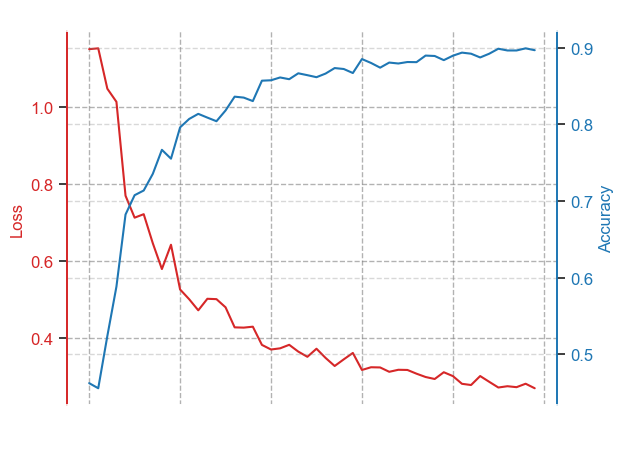
\includegraphics[width=0.65\textwidth]{VIT_loss-accuracy.png}
    \end{center}

    \small{
    \begin{cbox}
        \begin{itemize}
            \item Final training loss: $0.27$
            \item Final training accuracy: $90\%$
        \end{itemize}
    \end{cbox}
    }

\end{frame}

\begin{frame}
    
    \frametitle{Confidence and Test Accuracy}

    \begin{center}
        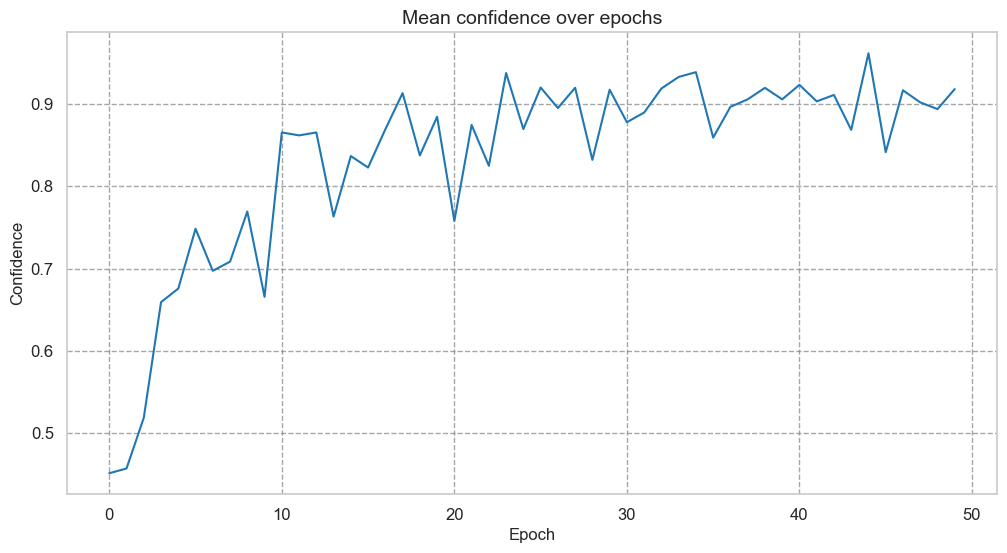
\includegraphics[width=0.65\textwidth]{VIT_confidence.png}
    \end{center}

    \small{
    \begin{cbox}
        \begin{itemize}
            \item Final training confidence: $96\%$
            \item Final test confidence: $93\%$
            \item \red{Final test accuracy: $88\%$}
        \end{itemize}
    \end{cbox}
    }

\end{frame}

\end{document}